%---------------------导言区---------------------------%
\documentclass[12pt,a4paper,UTF8]{ctexart}
	%10pt:正文字体为12pt,缺省为10pt;各层级字体大小会根据正文字体自动调整
	%a4paper:纸张大小a4;
	%UTF8:中文要求
\usepackage{geometry}%用于设置上下左右页边距
	\geometry{left=2.5cm,right=2.5cm,top=3.2cm,bottom=2.8cm}
\usepackage{xeCJK,amsmath,paralist,enumerate,booktabs,multirow,graphicx,subfig,setspace,listings,lastpage,hyperref,amssymb,upgreek}
	%xeCJK:中文字体(如楷体,作者和机构需要用到)的设置
	%amsmath:数学公式
	%paralist,enumerate:自定义项目符号
	%booktabs:三线图,论文常用的表格风格
	%multirow:复杂表格
	%graphicx,float: 插入图片
	%subfig:并排排版图片、竖向排版图片
	%setspace:设置行间距等功能
	\setlength{\parindent}{2em}%正文首行缩进两个汉字
	%listings:用于排版各种代码;比如matlab的代码
	\lstset{language=Matlab}%matlab代码
	%lastpage:获取总页数;
	%hyperref:超链接,和lastpage搭配.
\usepackage{fancyhdr}
	%fancyhdr:一个很强大的宏包,用于自定义设计页面风格并命名以供调用。
	\pagestyle{fancy}
	\rhead{实验 B9 迈克耳孙干涉及应用(白光干涉)}
	\lhead{基础物理实验\uppercase\expandafter{\romannumeral2}实验报告}
	\cfoot{Page \thepage/\pageref{LastPage}}  %当前页\总页数
		%分别是右页眉、左页眉、中页脚、右页脚
	\renewcommand{\headrulewidth}{0.4pt}
	\renewcommand{\theenumi}{(\arabic{enumi})}
	\setlength\headheight{15pt}

% \setCJKmainfont{FZShuSong-Z01S}[ItalicFont=FZKai-Z03S, BoldFont=FZHei-B01S]
%中文字体设置:使用开源字体方正书宋,方正楷体和方正黑体



%%%%%%%%%%%%%%%%%%%%%%%%%正文开始%%%%%%%%%%%%%%%%%%%%%%%%%%

\begin{document}

%%begin-------------------标题与信息-----------------------%%

%%标题
\begin{center}
\LARGE\textbf{实验 B9 迈克耳孙干涉及应用(白光干涉)}
\end{center}


%%end-------------------标题与信息-----------------------%%


\subsection*{【实验目的】}
	%*表示不带上小节本身应有的1.1,下面的subsubsection*也是一样
%%自定义项目符号之(1)(2)(3)
	\begin{enumerate}
		\item 观察等倾、等厚干涉现象及调节白光干涉条纹。
        \item 学习用迈克耳孙干涉仪测量钠光谱波长差的方法。
        \item 学习用白光干涉测量透明薄片折射率的方法。
	\end{enumerate}

\subsection*{【实验仪器】}
\begin{table}[htbp]
	\centering
	\begin{tabular}{cccp{20em}}
	\toprule
	编号    & 仪器用具名称 & 数量    & 主要参数(型号,测量范围,测量精度等) \\
	\midrule
	1     & 迈克耳孙干涉仪 & 1     &杭州精飞KF \\
	2     &钠灯 & 1 & KF-GP20Na \\
	3     & 透明薄片 & 1 & \\
	\bottomrule
	\end{tabular}%
	\label{tab:device}%
\end{table}%

\subsection*{【实验原理】}
\subsubsection*{1.利用白光干涉测定透明薄片的厚度或折射率}

\begin{figure}[htbp]
	\centering
	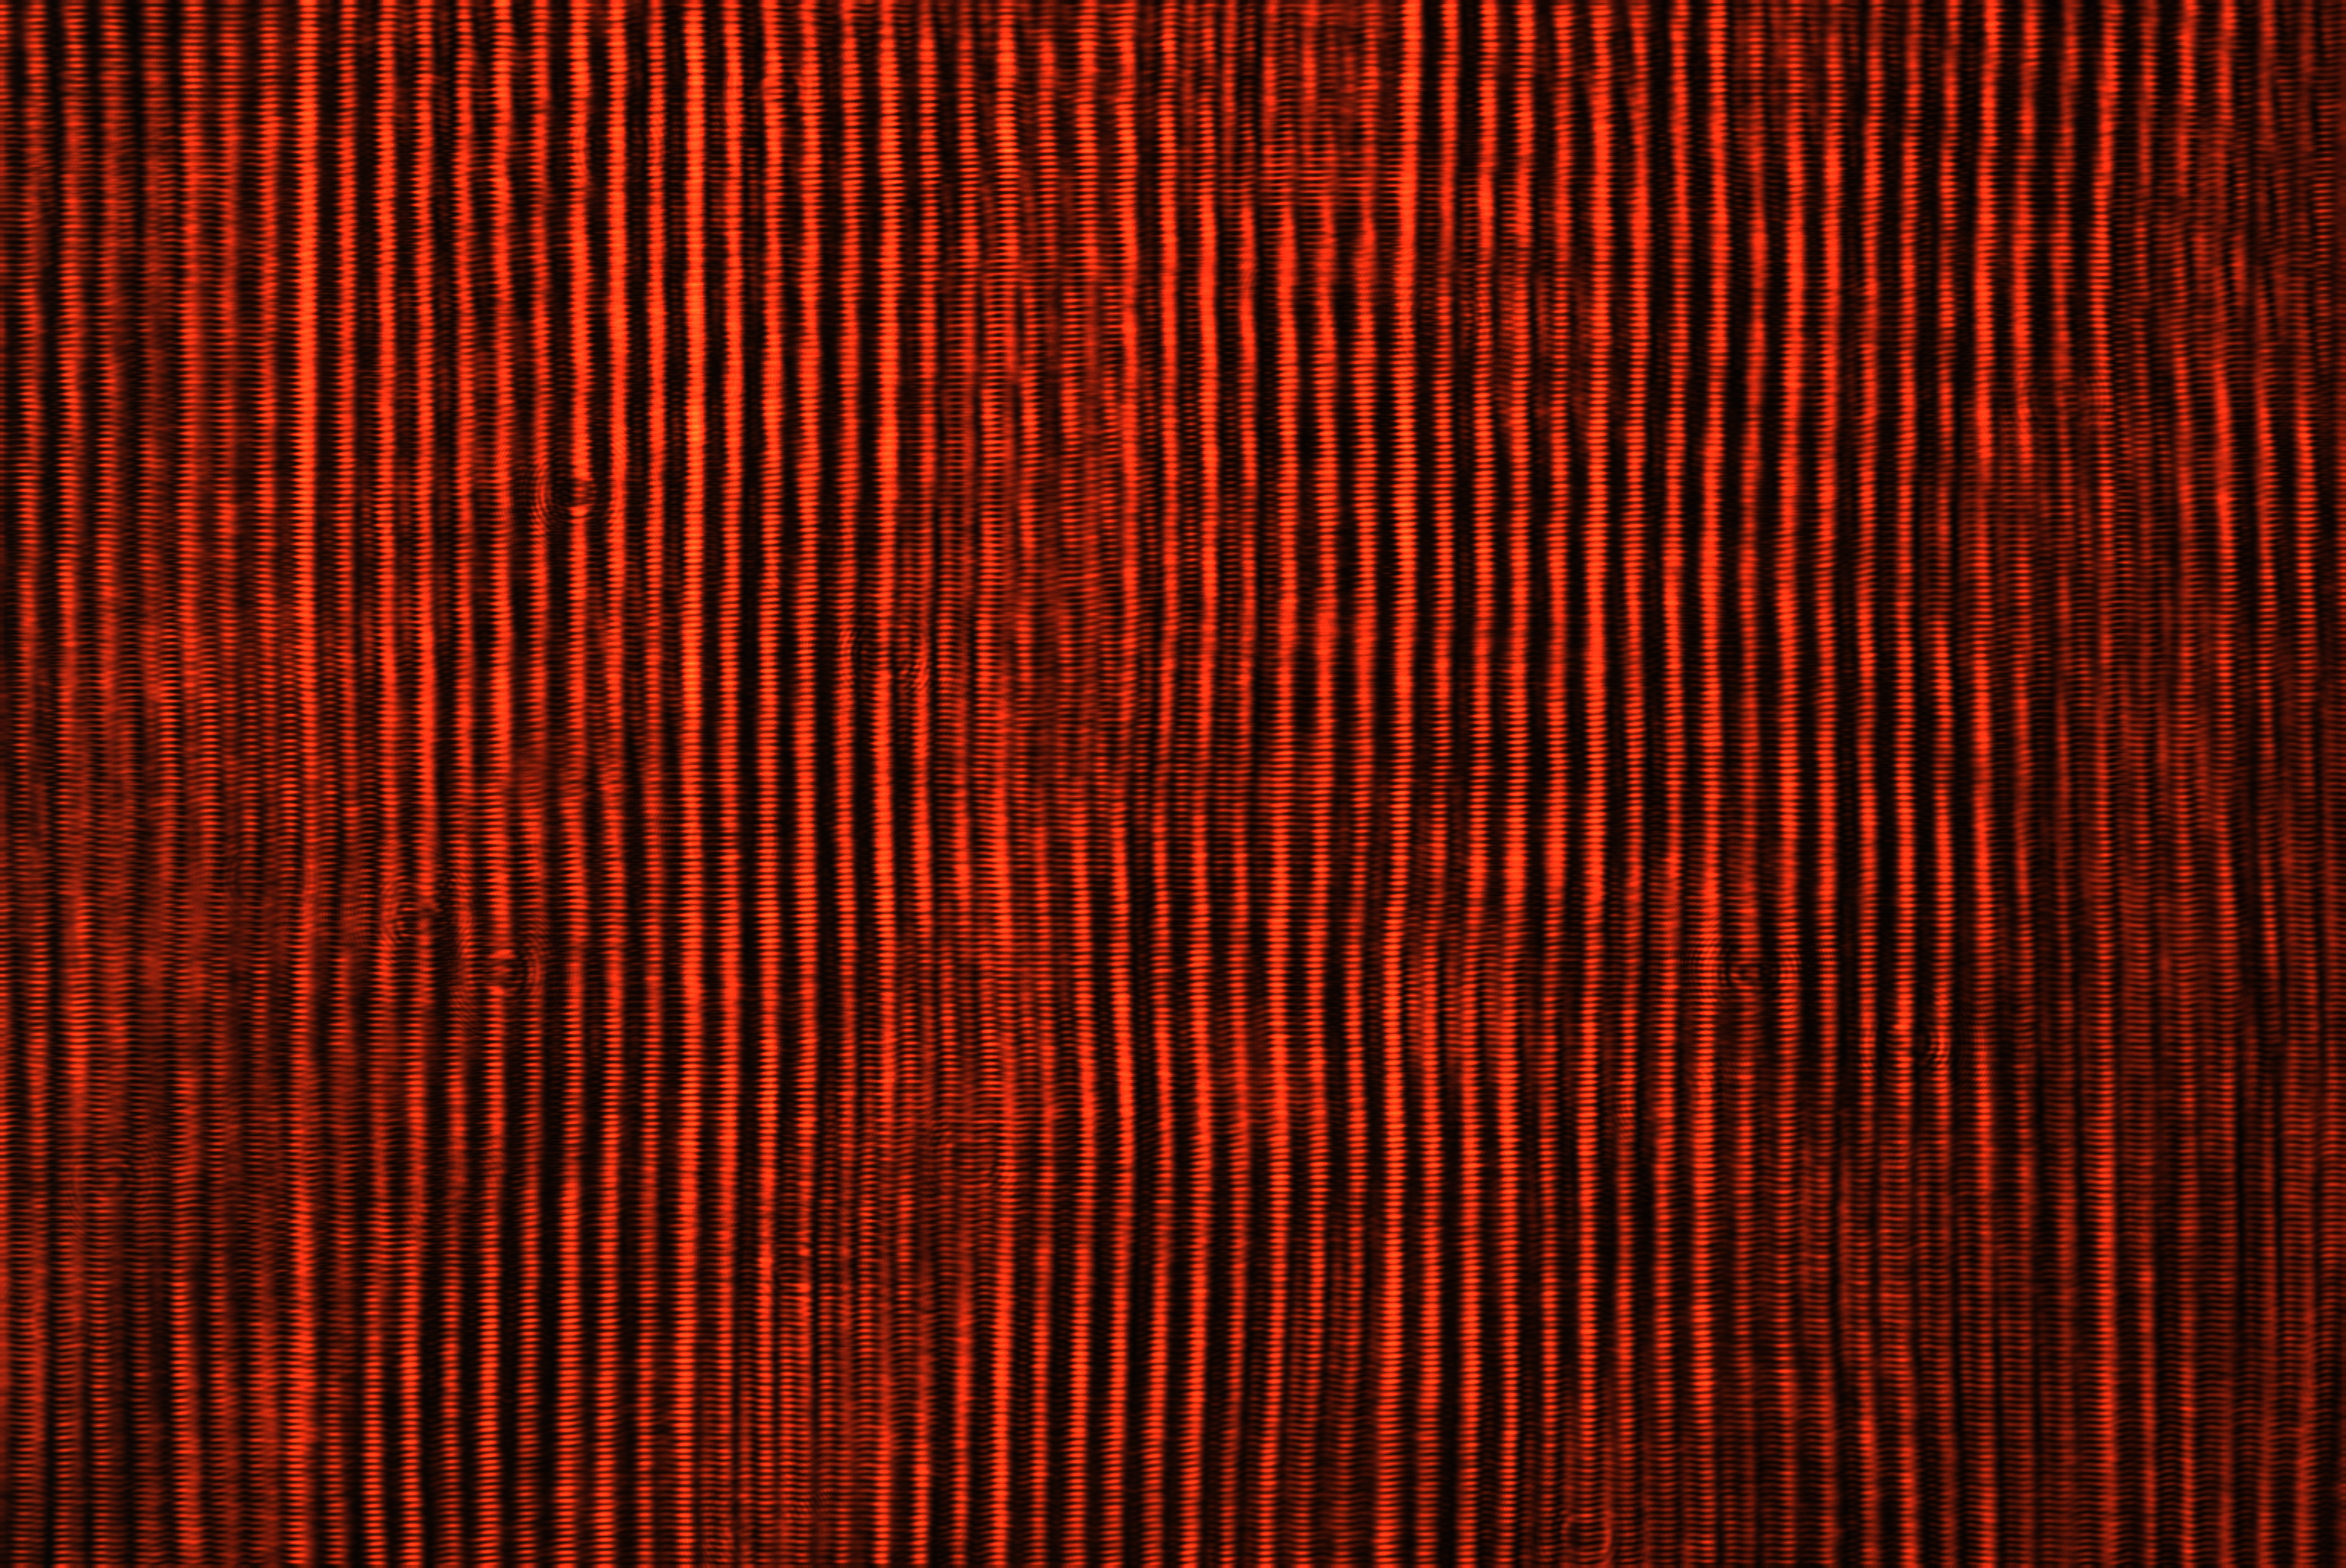
\includegraphics[width=0.6\textwidth]{img//1.jpg}
	\caption{迈克耳孙干涉仪原理}
\end{figure}


在迈克耳孙干涉实验中,如图A1所示的原理,若先采用激光光源,调节出等倾干
涉圆环,再减小两反射臂的光程差,直至等倾圆环几乎消失。这时如果换上扩散的白光光
源,并微调可调反射镜的倾斜度,则可在视场中观察到彩色的条纹,此即为白光等厚干涉
条纹,在彩色条纹的中间还可观察到一条全黑的条纹,称为中心暗纹,观察到此现象后,可
缓慢移动$M_1$镜,使中心暗纹移到视场中央,然后在$M_1$镜与分束镜$P_1$之间放上折射率为
n,厚度为t的透明薄片,且使薄片与$M_1$镜平行,则此时光程差要比原来增大
ΔL=2t(n-1).

白光彩色条纹随即移出视场范围,如果将$M_1$镜向前朝分束镜$P_1$方向移动一段距离
Δd,使Δd=Δl/2,则白光彩色干涉条纹重新出现(中心暗纹要移到视场中央),有
Δd=t(n-1).

测出$M_1$;镜的移动量Δd,若已知厚度,可求出折射率n;反之,若已知n,可求出t.

\subsubsection*{2.测钠双黄线的波长差}
钠黄光含有两种波长相近的光。若采用钠灯作光源,在干涉仅动镜$M_1$,移动过程中,
干涉条纹会出现清晰与模糊的周期性变化,称为光拍现象,设干涉条纹出现一次模糊到清晰后模糊的变化时,
$M_1$镜移动距离为Δd,则双钠黄线的波长差为$\delta\lambda =\frac {\overline{\lambda} ^{2}}{\delta d}$

\subsection*{【实验内容及步骤】}
\subsubsection*{结合说明书,学习精密干涉仪的调节方法,用HeNe激光器调节出等倾干涉条纹。}
    \begin{enumerate}
		\item 按图1安装干涉仪,扩束镜(2)先不安装。
		\item 调节He-Ne激光器的高度和倾斜度,使激光束从分束镜的中心入射。
		\item 调节$M_1$和$M_2$反射镜的倾斜度调节螺钉,使各镜面的人射和出射点高度与分束
		装接近,$M_1$和$M_2$反射的光点在观察屏中央重合。
		\item 装上扩束镜,观察干涉条纹。 
	\end{enumerate}

\subsubsection*{2.钠双黄线波长差的测量}
    \begin{enumerate}
		\item 用He-Ne激光,调出干涉圆环.移动反射镜$M_1$,使条纹变宽变稀,至观察屏上只
		有少数几个圆环,两干涉臂的光程几乎相等。
		\item 不安装扩束镜.改用钠灯,灯前装有毛玻璃使光散射,观察屏改为平面反射镜。
		\item 从反射镜中观察,仔细调节$M_2$镜后的倾斜度调节螺钉和$M_1$镜的位置,可观察
		到黄黑相间的直线状的等厚干涉条纹。
		\item 调节移动$M_1$,观察条纹模糊→清晰→模糊的周期变化过程,记录变化若干周期
		时M1镜移动的距离Δd.
		\item 计算钠双黄线的波长差。
	\end{enumerate}

\subsubsection*{3.白光干涉的调节并测透明薄片的折射率}
    \begin{enumerate}
		\item 用He-Ne激光,调出干涉圆环.移动反射镜$M_1$,使条纹变宽变稀,至观察屏上只
		有少数几个圆环,两干涉臂的光程几乎相等。
		\item 不安装扩束镜,改用汞灯,灯前装有毛玻璃使光散射,观察屏改为平面反射镜。
		\item 从反射镜中观察,仔细调节$M_2$镜后的倾斜度调节螺钉和$M_1$镜的位置,可观察
		\item 在分束镜$P_1$和动镜M1间安装透明薄片并与光路垂直,彩色条纹消失.缓慢调节
		到直线状的彩色干涉条纹。
		精密测微头,缩小$M_1$和$P_1$之间的距离,重新观察到彩色条纹,记录$M_1$移动的距离Δd.
		\item 用螺旋测微计测量薄片的厚度,计算薄片的折射率n.
	\end{enumerate}

\subsection*{【数据处理】}
\subsubsection*{1.钠双黄线波长差的测量}

\begin{table}[htbp]
	\centering
	\caption{实验数据记录}
	\begin{tabular}{ccccccc}
	\toprule
    模糊次数 & 1 & 2 & 3 & 4 & 5 & 6 \\
	\midrule
    $M_1$位置 d/mm &10.210 & 10.500 & 10.793 & 11.080 & 11.372 &11.661 \\
    $\varDelta d / mm $ & & 0.290 & 0.293 & 0.287 & 0.297 & 0.289 \\
	\bottomrule
	\end{tabular}%
	\label{tab:device}%
\end{table}%

\subsubsection*{计算波长差及误差}

查阅资料后可知Na 双黄线波长为
\begin{equation*}
    \lambda_1=589.0nm
\end{equation*}

\begin{equation*}
	\lambda_2=589.6nm
\end{equation*}

平均波长
\begin{equation*}
	\varDelta \overline{\lambda} =589.3nm
\end{equation*}

平均移动距离
\begin{equation*}
	\varDelta \overline{d}= \frac{1}{5}\sum_{i = 1}^{5}  d_i=\frac{1}{5} \times (0.290+0.293+0.287+0.297+0.289)=0.2912mm
\end{equation*} 

Na双黄线的波长差
\begin{equation*}
	\varDelta \lambda=\frac{\overline{\lambda}^{2}}{2\varDelta \overline{d}}=0.596nm
\end{equation*}

Na双黄线波长差理论值
\begin{equation*}
	\varDelta \lambda_0=0.600nm
\end{equation*}

相对误差 
\begin{equation*}
	E=\left\lvert \frac{\varDelta \lambda-\varDelta \lambda_0}{\varDelta \lambda_0}\right\rvert \times 100\%=0.6\%
\end{equation*}

\subsubsection*{计算不确定度}
平均值的实验标准差
\begin{equation*}
	S_{\varDelta d}=\sqrt{\frac{1}{n(n-1)}\sum_{i = 1}^{5}(\varDelta d_i-\varDelta \overline{d})^{2}} =0.0017mm
\end{equation*}

自由度
\begin{equation*}
	V_{\varDelta d}=n-1=4
\end{equation*}

A类不确定度
\begin{equation*}
	S_A=\sqrt{{\left( \frac{\partial \varDelta \lambda}{\partial \varDelta d}\times S_{\varDelta d}\right) }^2}=
	\sqrt{{\left( -\frac{\overline{\lambda}^2}{2 \varDelta d^2}\times S_{\varDelta d}\right) }^2}=0.0036nm
\end{equation*}

A类不确定度的自由度
\begin{equation*}
	V_A=\frac{S_A^4}{\left( \frac{\partial \varDelta \lambda}{\partial \varDelta d}\times S_{\varDelta d}\right) ^4 / V_{\varDelta d}}=4
\end{equation*}

\begin{equation*}
	U_{\varDelta d}=\frac{0.01mm}{\sqrt{3}}=0.00577mm
\end{equation*}

自由度$V_{U \varDelta d}=1$

B类不确定度
\begin{equation*}
	S_B=\sqrt{{\left( \frac{\partial \varDelta \lambda}{\partial \varDelta d}\times U_{\varDelta d}\right) }^2}=
	\sqrt{{\left( -\frac{\overline{\lambda}^2}{2 \varDelta d^2}\times U_{\varDelta d}\right) }^2}=0.0121nm
\end{equation*}

B类不确定度的自由度
\begin{equation*}
	V_B=\frac{S_B^4}{\left( \frac{\partial \varDelta \lambda}{\partial \varDelta d}\times U_{\varDelta d}\right) ^4 / V_{U \varDelta d}}=1
\end{equation*}

合成不确定度
\begin{equation*}
	S= \sqrt{S_A^2+S_B^2}=0.0127nm
\end{equation*}

合成自由度
\begin{equation*}
	V=\frac{S^4}{ \frac{S_A^4}{V_A}+ \frac{S_B^4}{V_B}}=1
\end{equation*}

取V=1,p=0.95,查表可得$t_p=12.71$

扩展不确定度为
\begin{equation*}
	\varDelta D=t_p S =0.15nm
\end{equation*}

计算结果为
\begin{equation*}
	\varDelta \lambda=\varDelta \overline{\lambda}\pm \varDelta D=(0.60\pm0.15)nm
\end{equation*}

\subsubsection*{误差分析}
1.人眼无法准确地做出清晰和模糊的界定,从而造成较大误差,可多次测量减小误差。

2.当实验中触碰桌子时,仪器会随之发生颤动,从而导致误差的产生。

\subsubsection*{2.白光干涉的调节并测透明薄片的折射率}

\begin{table}[htbp]
	\centering
	\caption{薄片厚度}
	\begin{tabular}{cccccccc}
	\toprule
    测量次数 & 1 & 2 & 3 & 4 & 5  & 均值 & 标准差\\
	\midrule
	薄片厚度/mm & 0.168 & 0.171 & 0.170 & 0.171 & 0.170 &0.170 &0.0005 \\
	\bottomrule
	\end{tabular}%
	\label{tab:device}%
\end{table}%

薄片平均厚度
\begin{equation*}
	\overline{t}= \frac{1}{5}\sum_{i = 1}^{5}  t_i=\frac{1}{5} \times (0.168 + 0.171 + 0.170 + 0.171 + 0.170 )=0.170mm
\end{equation*} 

平均厚度的实验标准差
\begin{equation*}
	S_{\varDelta t}=S_A=\sqrt{\frac{1}{n(n-1)}\sum_{i = 1}^{5}(\varDelta t_i-\varDelta \overline{t})^{2}} =0.00054mm
\end{equation*}

自由度
\begin{equation*}
	V_t=n-1=4
\end{equation*}

B类不确定度
\begin{equation*}
	S_B=\frac{0.01mm}{\sqrt{3}}=0.00577mm
\end{equation*}

B类自由度
\begin{equation*}
	V_B=1
\end{equation*}

合成不确定度
\begin{equation*}
	S= \sqrt{S_A^2+S_B^2}=0.0058mm
\end{equation*}

合成自由度
\begin{equation*}
	V=\frac{S^4}{ \frac{S_A^4}{V_A}+ \frac{S_B^4}{V_B}}=1
\end{equation*}

取V=1,p=0.95,查表可得$t_p=12.71$

测量结果为
\begin{equation*}
	\varDelta t=\varDelta \overline{t}\pm \varDelta N_{\varDelta t}=(0.17\pm0.07)mm
\end{equation*}


\begin{table}[htbp]
	\centering
	\caption{实验数据记录}
	\begin{tabular}{ccccccc}
	\toprule
    测量次数 & 1 & 2 & 3 & 4 & 5  \\
	\midrule
    模糊时$M_1$位置 $d_1/mm$ & 10.422 & 10.420 & 10.422 & 10.425 & 10.423 \\
    清晰时$M_1$位置 $d_2/mm $ & 10.321 & 10.322 & 10.323 & 10.323 & 10.320 \\
	$\varDelta d /mm$ & 0.101 & 0.098 & 0.099 & 0.102 & 0.103 \\
	\bottomrule
	\end{tabular}%
	\label{tab:device}%
\end{table}%

平均移动距离
\begin{equation*}
	\varDelta \overline{d}= \frac{1}{5}\sum_{i = 1}^{5}  d_i=\frac{1}{5} \times (0.101 + 0.098 + 0.099 + 0.102 + 0.103)=0.1006mm
\end{equation*} 

平均值的实验标准差
\begin{equation*}
	S_{\varDelta d}=\sqrt{\frac{1}{n(n-1)}\sum_{i = 1}^{5}(\varDelta d_i-\varDelta \overline{d})^{2}} =0.0009mm
\end{equation*}

自由度
\begin{equation*}
	V_{\varDelta d}=n-1=4
\end{equation*}

由公式得
\begin{equation*}
	n=\frac{\varDelta d}{t}+1
\end{equation*}

n均值为
\begin{equation*}
	\overline{n}=\frac{\varDelta\overline{d}}{\overline{t}}+1=1.592
\end{equation*}


A类不确定度
\begin{equation*}
	S_A=\sqrt{{\left( \frac{\partial n}{\partial \varDelta d}\times S_{\varDelta d}\right) }^2+{\left( \frac{\partial n}{\partial t}\times S_{t}\right) }^2}=
	\sqrt{{\left( -\frac{1}{\overline{t}}\times S_{\varDelta d}\right) }^2+{\left( -\frac{\varDelta\overline{d}}{\overline{t}^2}\times S_{t}\right) }^2}=0.00578
\end{equation*}

A类不确定度的自由度
\begin{equation*}
	V_A=\frac{S_A^4}{{\left( \frac{\partial n}{\partial \varDelta d}\times S_{\varDelta d}\right) }^4/V_{\varDelta d}+{\left( \frac{\partial n}{\partial t}\times S_{t}\right) }^4/V_t}=4.96
\end{equation*}

\begin{equation*}
	U_{\varDelta d}=\frac{0.01mm}{\sqrt{3}}=0.00577mm
\end{equation*}

自由度$V_{U \varDelta d}=1$

B类不确定度
\begin{equation*}
	S_B=\sqrt{{\left( \frac{\partial n}{\partial \varDelta d}\times U_{\varDelta d}\right) }^2+{\left( \frac{\partial n}{\partial t}\times U_{t}\right) }^2}=
	\sqrt{{\left( -\frac{1}{\overline{t}}\times U_{\varDelta d}\right) }^2+{\left( -\frac{\varDelta\overline{d}}{\overline{t}^2}\times U_{t}\right) }^2}=0.039
\end{equation*}

B类不确定度的自由度
\begin{equation*}
	V_B=\frac{S_B^4}{{\left( \frac{\partial n}{\partial \varDelta d}\times U_{\varDelta d}\right) }^4/V_{\varDelta d}+{\left( \frac{\partial n}{\partial t}\times U_{t}\right) }^4/V_t}=1.62
\end{equation*}

合成不确定度
\begin{equation*}
	S= \sqrt{S_A^2+S_B^2}=0.04
\end{equation*}

合成自由度
\begin{equation*}
	V=\frac{S^4}{ \frac{S_A^4}{V_A}+ \frac{S_B^4}{V_B}}=1.69
\end{equation*}

取V=2,p=0.95,查表可得$t_p=4.3$

扩展不确定度为
\begin{equation*}
	\varDelta n=t_p S =0.17
\end{equation*}

计算结果为
\begin{equation*}
	n=\overline{n} \pm \varDelta n=1.59\pm0.17
\end{equation*}

\subsubsection*{误差分析}
1.由于条纹较浅,故清晰与模糊的边界难以用肉眼准确分辨,从而造成较大的误差

2.薄片厚度测量时最后一位是估读数,存在一定误差。

3.薄片不一定与光路严格垂直,导致实验中厚度增加,测量的折射率增大。


\newpage
\subsection*{【思考题】}
\subsubsection*{(1)如何测量透明溶液的折射率?请提出实验方案并说明其合理性。}
答:实验方案:
(1)安装干涉仪,在分束镜和$M_1$镜之间放一个透明容器并与光路垂直(先不安装扩束镜)。
(2)调节He-Ne激光器的高度和倾斜度,使激光束从分束镜的中心入射。
(3)调节 $M_1$ 和 $M_2$ 反射镜的倾斜度调节螺钉,使各镜面的入射和出射点高度与分束镜接近, $M_1$ 和 $M_2$
反射的光点在观察屏中央重合。
(4)装上扩束镜,观察干涉条纹。移动反射镜$M_1$,使条纹变宽变稀,至观察屏上只有少数几个圆环,两个
干涉臂的光程几乎相等。
(5)撤下扩束镜。把激光器换成汞灯,灯前装有毛玻璃使光散射。将观察屏的一面换成平面反射镜。
(6)从反射镜中观察,仔细调节$M_2$镜后的倾斜度调节螺钉和$M_1$镜的位置,直至观察到直线状的彩色
干涉条纹。
(7)在分束镜$P_1$和动镜$M_1$间的透明容器中加所需测液体并与光路垂直,彩色条纹消失。缓慢调节精
密测微头,缓慢调节精密测微头,缩小$M_1$和$P_1$之间的距离,重新观察到彩色条纹,记录$M_1$移动的距离$\varDelta d$.
(8)用螺旋测微器测量容器的厚度,根据式$n=\varDelta d/(t+1)$计算透明溶液的折射率n.

\subsubsection*{(2)当空气的温度改变时,空气的折射率也会改变的,怎样去测量空气的折射率?}
答:空气折射率会随空气状态改变而改变,我们可以利用基于传感器的空气折射率测量仪测量空气折射
率:将常温下测得的空气温度、压力和相对湿度,利用HP03MA传感器以及相应计算机程序读取补偿系数、
温度及压力值,对温度和压力值进行修正后代入Edlen经验公式,最终计算出空气折射率n.HP03MA系统
的主要功能是从一个压力传感器转换为补偿压力和温度信号。转换后可得到D1(测量气压)和D2(测量温
度)值。因为传感器是随着温度强烈变化的,所以必须对这些影响进行一些补偿。HP03MA传感器中需要赋
予补偿系数特定的输入值,压力(单位:0.01hpA)和温度(单位:0.1°C)作为输出值。


\end{document}
